\section{Instruction set}
There was a minimal instruction set required to complete this assignment which was implemented in \emph{processor.vhd}:
\begin{itemize}
    \item Several ALU instructions (all working on two registers and storing the result in a third):
        \begin{itemize}
            \item ADD - Addition
            \item SUB - Subtraction
            \item SLT - Store 1 in destination if the first source register is less than second
            \item AND - Bitwise and
            \item OR  - Logical or
        \end{itemize}
    \item BEQ - branch if registers are equal
    \item LW - Load word from memory
    \item SW - Store word to memory
    \item LUI - Store immediate value shifted left 16 bits in a register
    \item J - Jump
\end{itemize}

\section{Architecture}
\begin{figure}[ht]
    \centering
    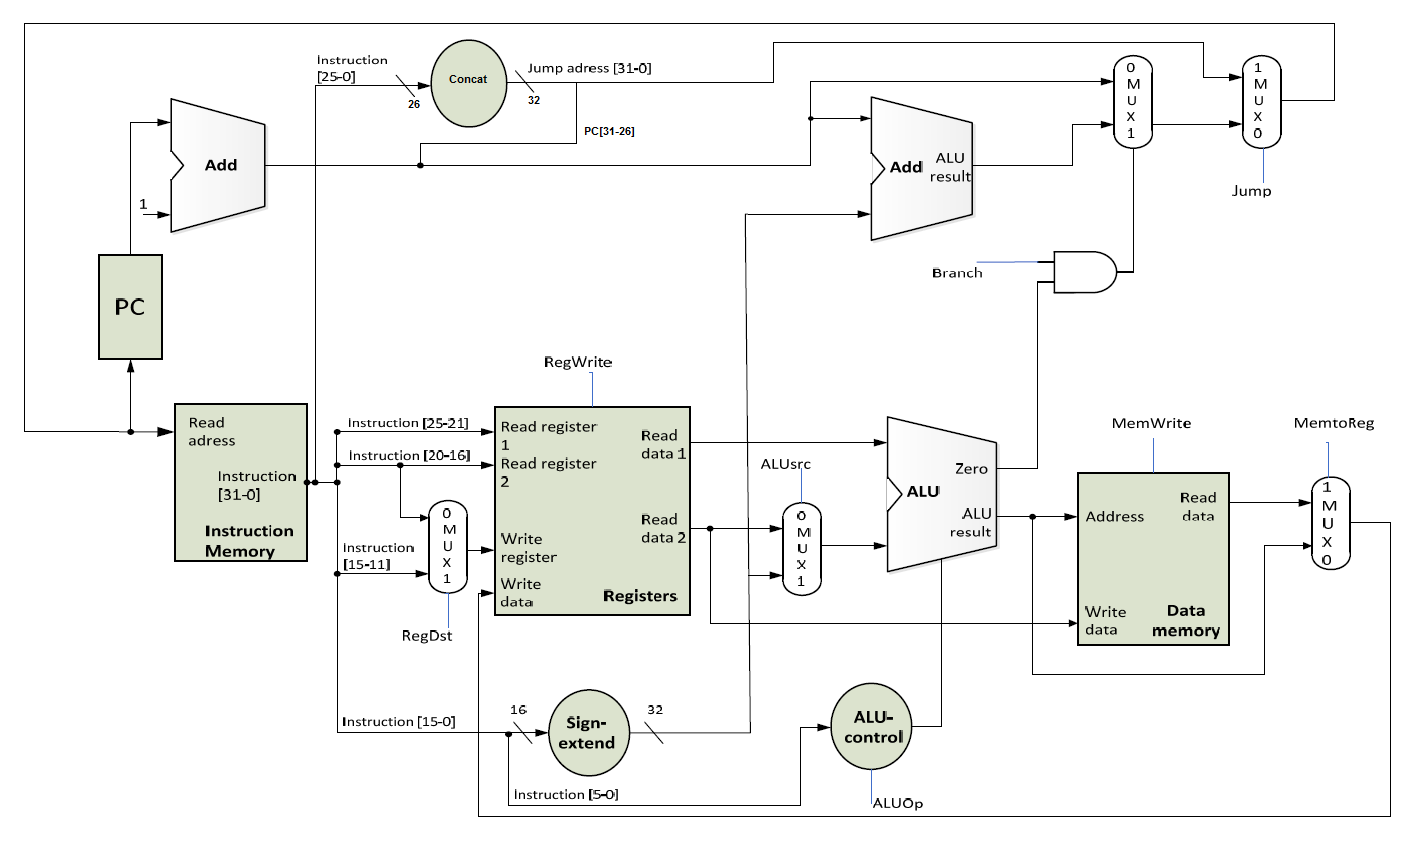
\includegraphics[scale=0.3]{figures/cpu.png}
    \caption{\label{fig:cpuArchitecture}The implemented CPU architecture.} 
\end{figure}

The suggested CPU architecture remained mostly unchanged.
The main difference is that instead of retrieving the instruction address from the program counter, %TODO: reference, page 115 compendium
it is retrieved directly from the same bus that is used to set the program
counter. This is because it shouldn't take another clock cycle to start the
execution.

\subsection{The control unit}
\begin{figure}[ht]
    \centering
    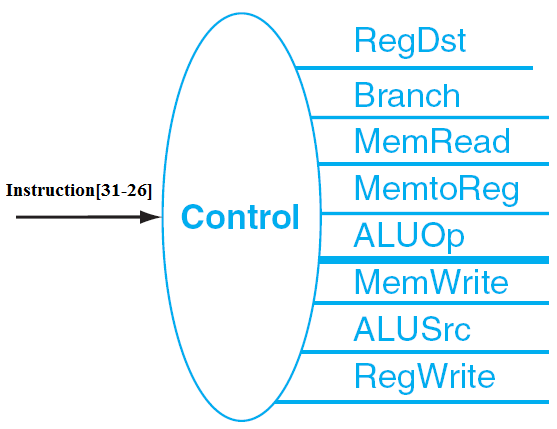
\includegraphics[scale=0.3]{figures/controlunit.png}
    \caption{\label{fig:controlUnit}The control unit.}
\end{figure}
The control unit was implemented as a state machine, a decoder and a splitter.
On a rising clock edge, it will update it's state depending on its current
state. These can be fetch, where the instruction is fetched from the data bus
and the program counter is updated before the state is set to execute, or it can
be execute, where the CU lets the CPU do its thing before setting the state to
the next, or finally stall, where only the next instruction is fetched.
Figure \ref{fig:stateMachine} shows how the machine can move between the states. If none
of these states are the current state, something weird has gone wrong, and the
CU stalls. This is only a sanity check, and should not happen.

\begin{figure}[ht]
    \centering
    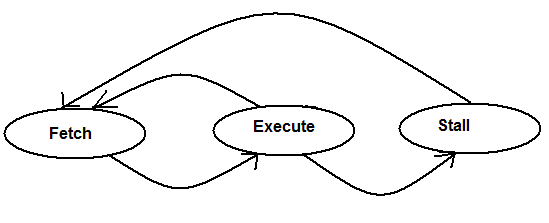
\includegraphics[scale=0.5]{figures/controlunitstatemachine.png}
    \caption{\label{fig:stateMachine}The state machine}
\end{figure}



The splitter simply splits the instruction into various signals from the IMEM
bus. The decoder is the process that prepares for the executions of the
instructions. It has a switch statement distinguishing between the various
opcodes, and setting the correct control signals depending on the code. 
